\section{Piedra Moreno Alitza Alejandra}
\subsection{Definiciones}

\subsubsection{Latex}
LaTeX es un sistema de composición de textos, orientado especialmente a la creación de libros, documentos científicos y técnicos que contengan fórmulas matemáticas.

LaTeX está formado por un gran conjunto de macros de TeX, escrito por Leslie Lamport en 1984, con la intención de facilitar el uso del lenguaje de composición tipográfica, TeX. Es muy utilizado para la composición de artículos académicos, tesis y libros técnicos, dado que la calidad tipográfica de los documentos realizados con LaTeX es comparable a la de una editorial científica de primera línea.
\cite{Dlsi.ua.es}

\subsubsection{Github}

GitHub es una plataforma de alojamiento, propiedad de Microsoft, que ofrece a los desarrolladores la posibilidad de crear repositorios de código y guardarlos en la nube de forma segura, usando un sistema de control de versiones llamado Git.

Facilita la organización de proyectos y permite la colaboración de varios desarrolladores en tiempo real. Es decir, nos permite centralizar el contenido del repositorio para poder colaborar con los otros miembros de nuestra organización.
\cite{Platzi}

\subsubsection{Git}

Git es un sistema de control de versiones distribuido, lo que significa que un clon local del proyecto es un repositorio de control de versiones completo. Estos repositorios locales plenamente funcionales permiten trabajar sin conexión o de forma remota con facilidad.

\cite{Microsoft}

\subsubsection{Visual studio code}

Visual Studio Code (VS Code) es un editor de código fuente desarrollado por Microsoft. Es software libre y multiplataforma, está disponible para Windows, GNU/Linux y macOS. VS Code tiene una buena integración con Git, cuenta con soporte para depuración de código, y dispone de un sinnúmero de extensiones, que básicamente te da la posibilidad de escribir y ejecutar código en cualquier lenguaje de programación.\cite{OpenWebinars.net}

\subsubsection{Estudio de movimientos}

Implica el análisis cuidadoso de cada uno de los movimientos corporales que se emplean para realizar una tarea. 
\cite{niebel1980ingenieria}
Es el análisis de métodos, materiales, herramientas, e instalación utilizada o que se ha de utilizar en la ejecución de un trabajo.

\subsubsection{Movimientos básicos} 
Como parte del análisis de movimientos, los Gilbreth concluyeron que todo trabajo, ya sea productivo o no, se realiza mediante el uso de combinaciones de 17 movimientos básicos a los que ellos llamaron therblig \cite{niebel1980ingenieria}  

Estos se dividen en eficientes, que estimulan el progreso del trabajo y con frecuencia pueden ser acortados, pero por lo general no pueden ser eliminados:
\begin{enumerate}
    \item \textbf{Alcanzar (AL):} “Mover” la mano vacía hacia o desde el objeto; donde el tiempo depende de la distancia recorrida.
    \item \textbf{Mover (M):} “Mover” la mano cargada; el tiempo depende de la distancia, el peso y el tipo de movimiento.
    \item \textbf{Tomar (T):} “Cerrar” los dedos alrededor de un objeto, este comienza cuando los dedos tocan el objeto y termina cuando se ha ganado el control.
    \item \textbf{Soltar (SL):} “Soltar” el control de un objeto, normalmente el más corto de los therbligs.
    \item \textbf{Preposicionar (PP):} ”Posicionar” un objeto en una ubicación predeterminada para su uso posterior. Por lo general ocurre en conjunto con “Mover”.
    \item \textbf{Utilizar (U):} “Manipular” Una herramienta para el uso por el que fue diseñada; fácilmente detectable a medida que avanza el progreso del trabajo.
    \item \textbf{Ensamblar (E):} “Unir” dos partes que embonan. Por lo general es precedido por “Posicionar” o “Mover” y seguido por “Liberar”.
	\item \textbf{Desensamblar (DE):} Es lo opuesto a “Ensamblar”, pues separa partes que embonan.

 También encontramos los ineficientes, los cuales no representan un avance en el proceso del trabajo y debe eliminarse. En esta categoría encontraremos:

    \item \textbf{Buscar (B):} Ojos o manos buscan un objeto; comienza a medida que los ojos se mueven para localizar un objeto.
    \item \textbf{Seleccionar (SE):} “Mover” la mano cargada; el tiempo depende de la distancia. Por lo general es seguido por “Buscar”.
    \item \textbf{Sostener (SO):} Una mano soporta el objeto mientras la otra realiza trabajo útil.
    \item \textbf{Posicionar (P):} “Orientar” un objeto durante el trabajo, por lo general precedido por “Mover” y seguido por “liberar”.
    \item \textbf{Inspeccionar (I):} “Comparar” un objeto con el estándar, típicamente a la vista, pero podría ser también con los demás sentidos.
    \item \textbf{Planear (PL):} “Pausar” para determinar la acción siguiente; por lo general se le detecta como un titubeo que precede a “Mover”
    \item \textbf{Retraso Inevitable (DI):} Más allá del control de quien opera debido a la naturaleza de la operación.
    \item \textbf{Retraso Evitable (DEV):} Quien opera es único/a responsable del tiempo ocio.
    \item \textbf{Descansar (DES):} Aparece periódicamente, no en cada ciclo. Depende de la carga de trabajo física.

\end{enumerate}

\subsubsection{Sistemas de tiempo predeterminado}

Conjunto de reglas o métodos para determinar con anticipación la secuencia de sucesos.

\subsubsection{Métodos de medición del tiempo}

 Es un sistema estandarizado para medir los tiempos que tardan los trabajadores en ejecutar una tarea repetitiva. El objetivo de este sistema es analizar donde están los movimientos ineficaces que se traducen en pérdidas innecesarias de tiempo en una tarea que se ejecuta cientos de veces al día. \cite{DanielGrifol}

\subsubsection{Precisión}

La precisión es lograr la mínima dispersión al momento de hacer una medición o de realizar una tarea. Es la variación o poca variación significa un buen grado de precisión.

\subsubsection{Exactitud}

Se define con respecto a su cercanía o sesgo, mayor cercanía implica un buen grado de exactitud.

\subsubsection{Muestreo}

Acción de escoger muestras representativas de calidad que describa de manera exacta las características de un conjunto que nos dejen deducir, inferir y sacar conclusiones de un fenómeno a estudiar. \cite{RAE}

\subsubsection{Representativo}

Significativo, característico, peculiar, relevante e importante. \cite{RAE}

\subsubsection{Inferir}

Deducir algo o sacarlo de conclusión de otra cosa.\cite{RAE}

\subsubsection{Muestreo de trabajo}

Lo podemos considerar como una herramienta para disminuir el costo que se presenta  en el estudio continuo del tiempo. Su único problema es obtener una muestra representativa.

\subsubsection{Estudio de tiempos convencional}

Es una muestra continua de n ciclos suponiendo que la distribución estadística es normal.

\subsubsection{Estudio de tiempos no convencional}

Esta contiene huecos entre las lecturas de muestreo y es una muestra discreta suponiendo que la distribución estadística es binomial.

\subsubsection{Tiempo productivo}

El tiempo productivo es la calificación del desempeño de operador, está basada en la experiencia, capacitación y juicio del analista que lo realiza.

\subsubsection{Diagrama de procesos de bimanual}

Herramienta que muestra todos los movimientos y retrasos atribuibles a las manos derecha e izquierda, además de la relación que existe entre ellas. 
Tiene como propósito identificar los patrones de movimiento que resultan ineficientes y observar las violaciones a los principios de la economía de movimientos.\cite{niebel1980ingenieria}

\subsubsection{Colocación de las herramientas y materiales}

En cada movimiento que se realiza está involucrada una distancia, a medida que la distancia es mayor, el esfuerzo muscular, el control y el tiempo serán mayores. Por ello, minimizar las distancias es lo que se busca.

El área de trabajo normal en el plano horizontal de la mano tanto derecha e izquierda incluye el área circunscrita por el brazo bajo el codo cuando se mueve para formar un arco que gira con respecto al codo.

Esta representa la zona más conveniente dentro de la cual es más cómodo realizar movimientos con la mano y no consumirá más energía de la requerida. El área máxima es la zona que  comprende un movimiento más amplio de los brazos, es decir, el área virtual que abarcan los brazos al hacer un “barrido” y completamente extendidos. Entendiendo que el área máxima será para aquellos elementos que se usan con una frecuencia menor, en un promedio de 3 veces por hora, pues esta zona depende de un movimiento más amplio. \cite{niebel1980ingenieria}

\subsubsection{Equipo para el estudio de tiempos}

El equipo mínimo requerido para realizar un programa de estudio de tiempos incluye un cronómetro, un tablero de estudio de tiempos, las formas para el estudio y una calculadora de bolsillo. Un equipo de videograbación también puede ser muy útil.

\textbf{Cronometro}
Reloj de gran precisión para medir fracciones de tiempo muy pequeñas, utilizado en industria y en competiciones deportivas.
\cite{RAE}

\textbf{Cámaras de videograbación}
Las cámaras de videograbación son ideales para grabar los métodos del operario y el tiempo transcurrido. Al tomar película de la operación y después estudiarla cuadro por cuadro, los analistas pueden registrar los detalles exactos del método usado y después asignar valores de tiempos normales. 

\textbf{Tablero de estudio de tiempos}

Los analistas encuentran conveniente tener un tablero adecuado para sostener el estudio de tiempos y el cronómetro. El tablero debe ser ligero, fuerte y suficientemente duro para proporcionar el apoyo necesario para la forma de estudio de tiempos. El tablero debe tener contactos para el brazo y el cuerpo con el propósito de que el ajuste sea cómodo y resulte fácil escribir mientras se sostiene.

\textbf{Forma de estudio de tiempo}

En una forma de estudios se registra toda la información pertinente sobre el método que se estudia, las herramientas utilizadas, etc. La operación en estudio se identifica mediante información como nombre y número del operario, descripción y número de la operación, nombre y número de la máquina, herramientas especiales usadas y sus números respectivos, el departamento donde se realiza la operación y las condiciones de trabajo prevalecientes. 
\cite{niebel1980ingenieria}

\subsubsection{Ciclos en el estudio}
 Como el estudio de tiempos es un procedimiento de muestreo, se puede suponer que las observaciones se distribuyen normalmente respecto a una media poblacional desconocida con una varianza desconocida. Si se usa la media muestral y la desviación estándar muestral s, la distribución normal para una muestra grande lleva al siguiente intervalo de confianza.

\begin{center} 

${\-x}+-{\frac{zs}{\sqrt{n}}}$

\end{center}

\subsection{Materiales}

\begin{center}

\begin{tabular}{ |p{1.5cm}|p{4cm}|p{4cm}|p{5cm}| }

\hline
\multicolumn{4}{|c|}{Lista de materiales} \\

 
\hline
 No.  & Nombre  & Figura  & Foto \\
\hline
 PC-01  & Almohadilla & \centering   & \\
\hline
 PC-02  & Protoboard & \centering  & \\
\hline
 PC-03 & LCD 16X2  & \begin{center}
     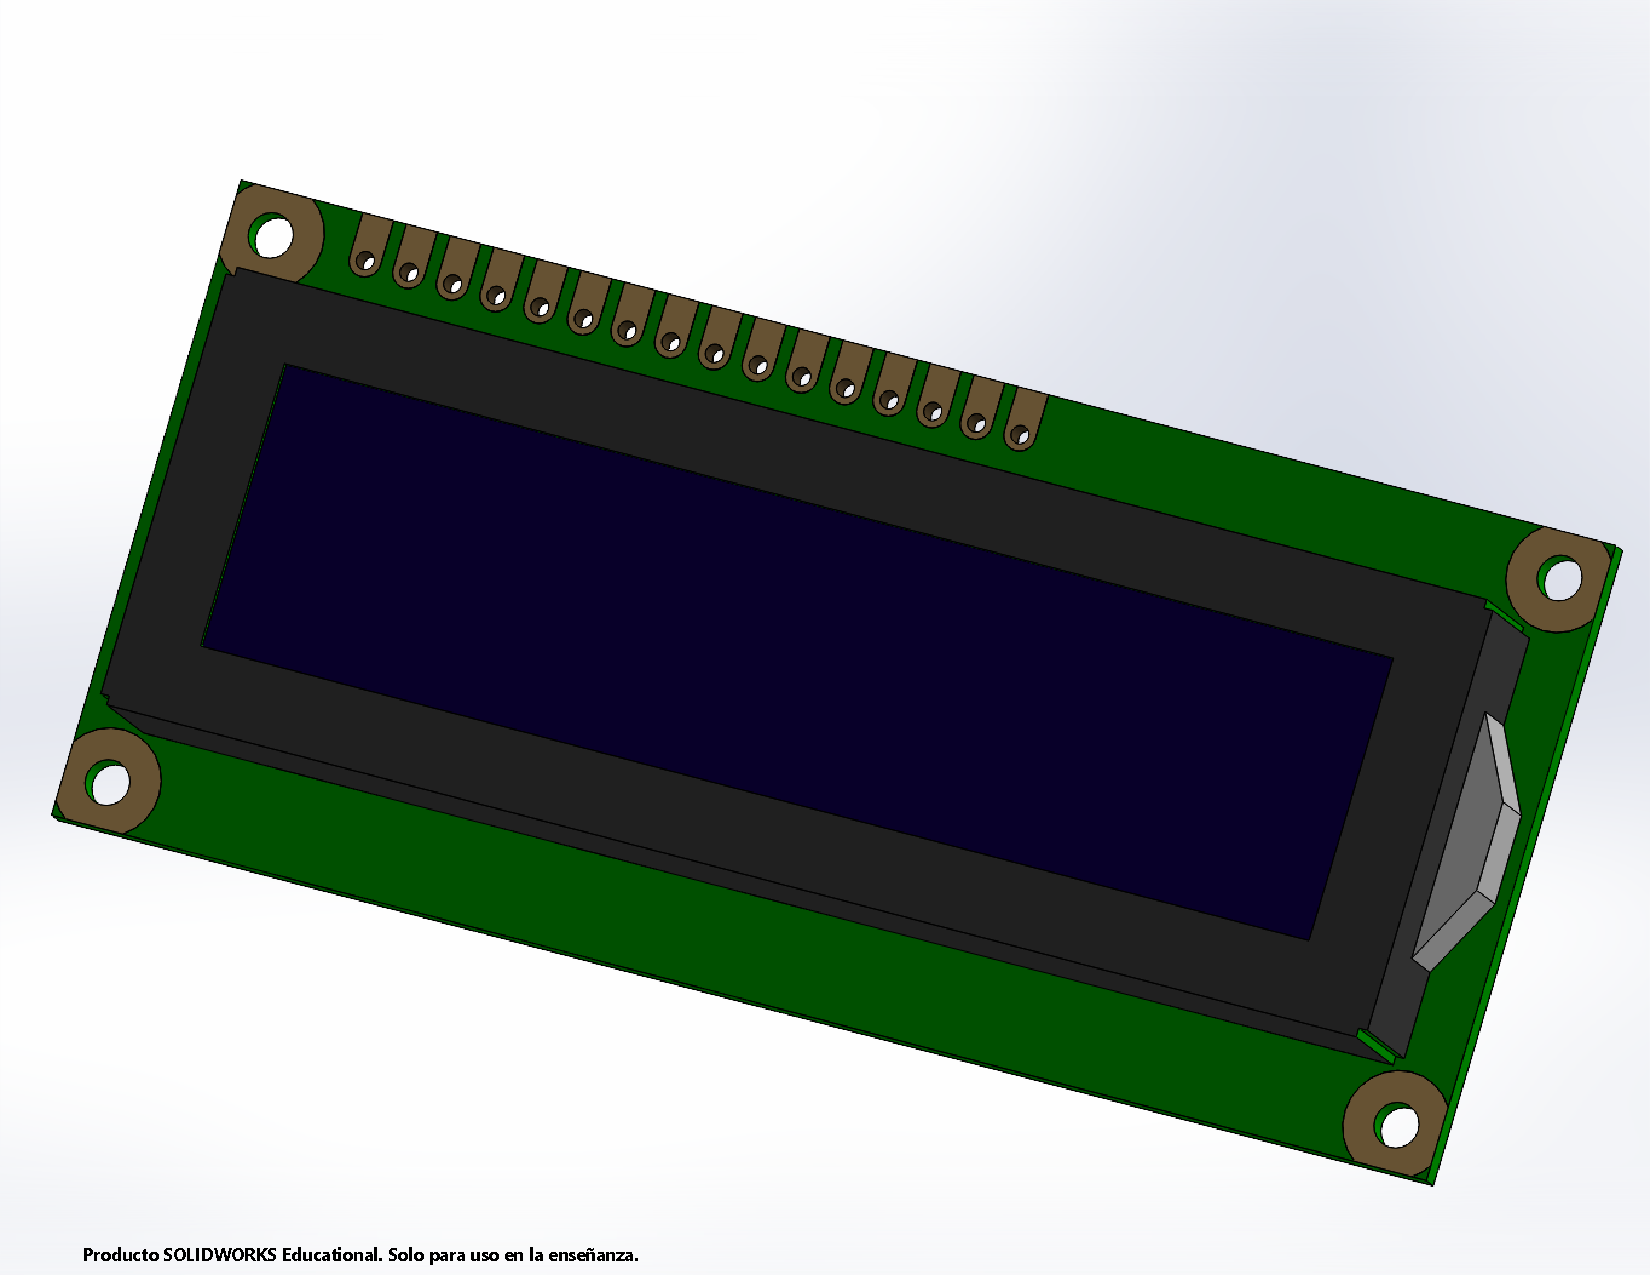
\includegraphics[width=.2\textwidth]{22/img/lcdFigura.PDF}~\\[5cm]  \end{center}   & \\
\hline
 PC-04  & Adaptador de LCD  & \begin{center}
     \includegraphics[width=.2\textwidth]{22/img/móduloI2CInterfazFigura.PDF}~\\[5cm]  \end{center}  & \\
\hline
 PC-05 & ESP32  & \begin{center}
     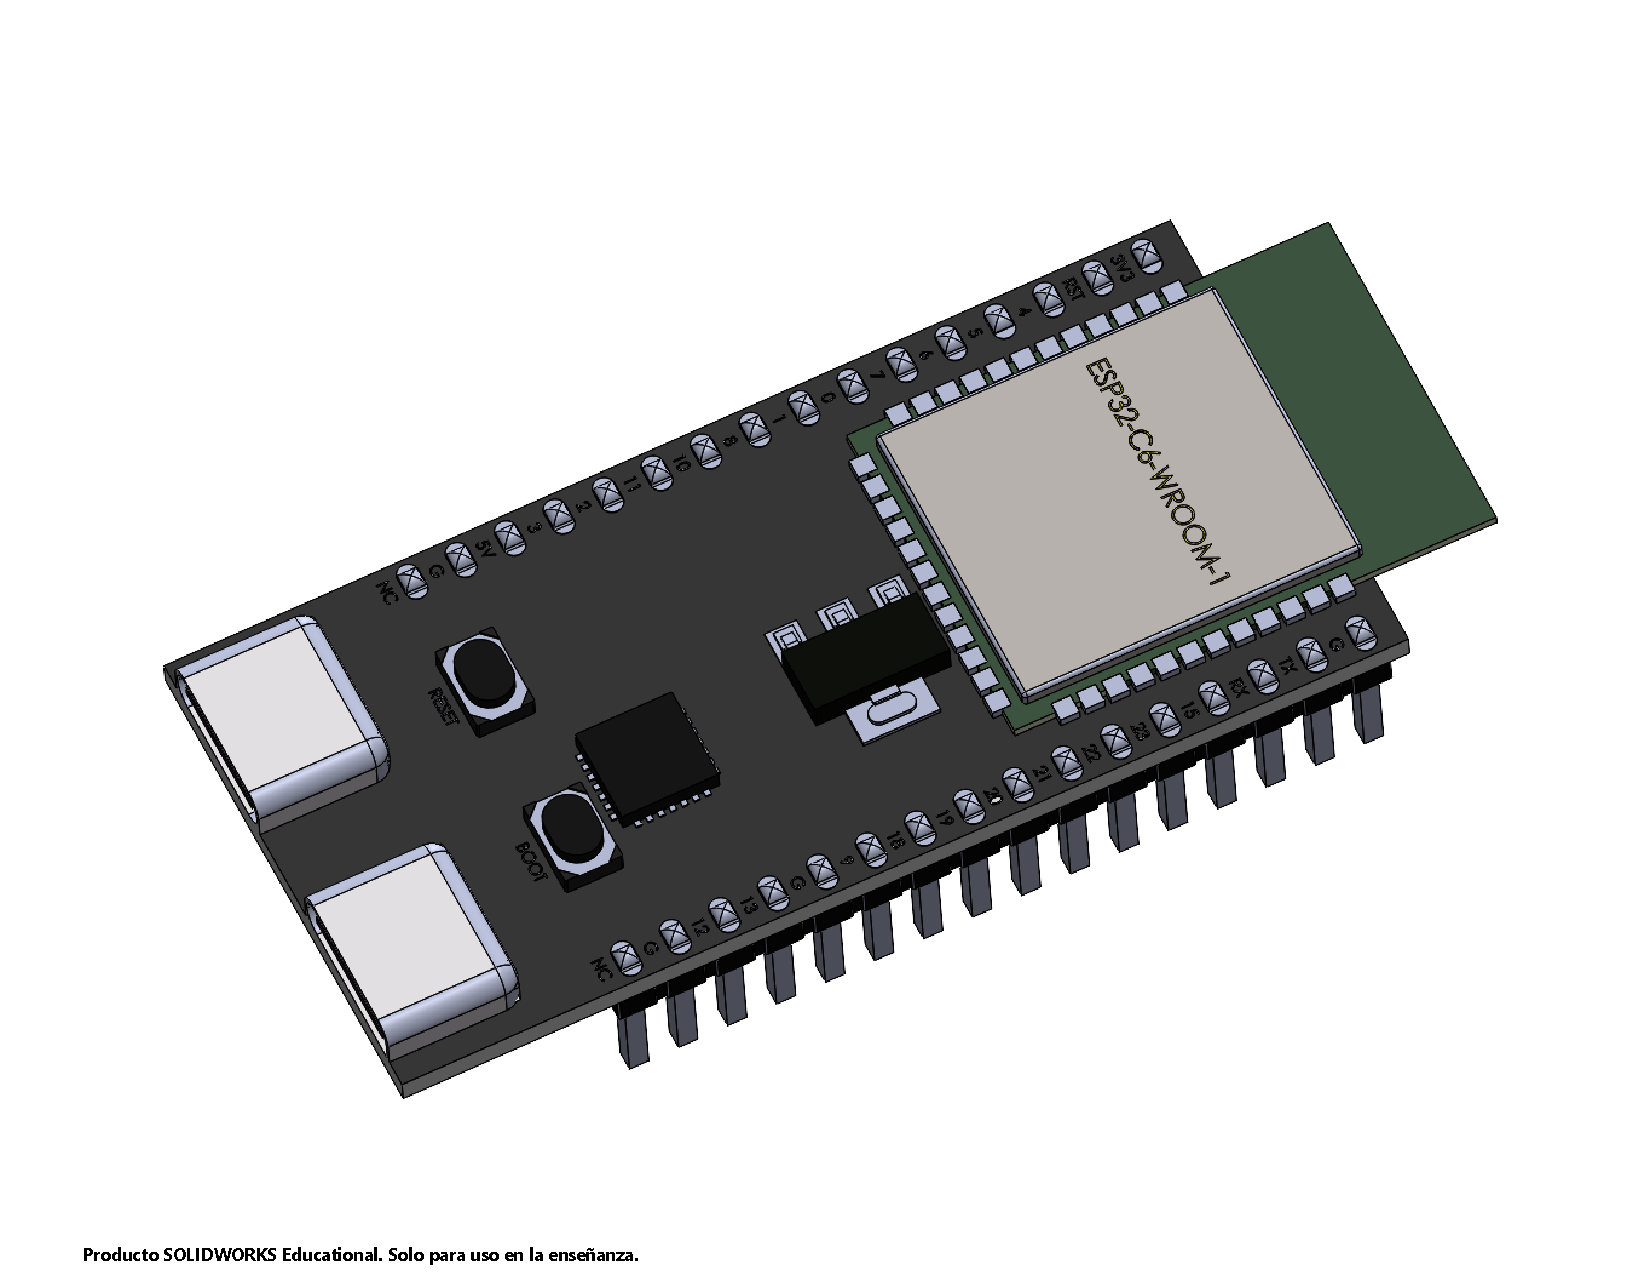
\includegraphics[width=.2\textwidth]{22/img/esp32Figura.PDF}~\\[5cm]  \end{center} &  \\
\hline 
 PC-06  & Potenciómetro  & \centering \begin{center}
     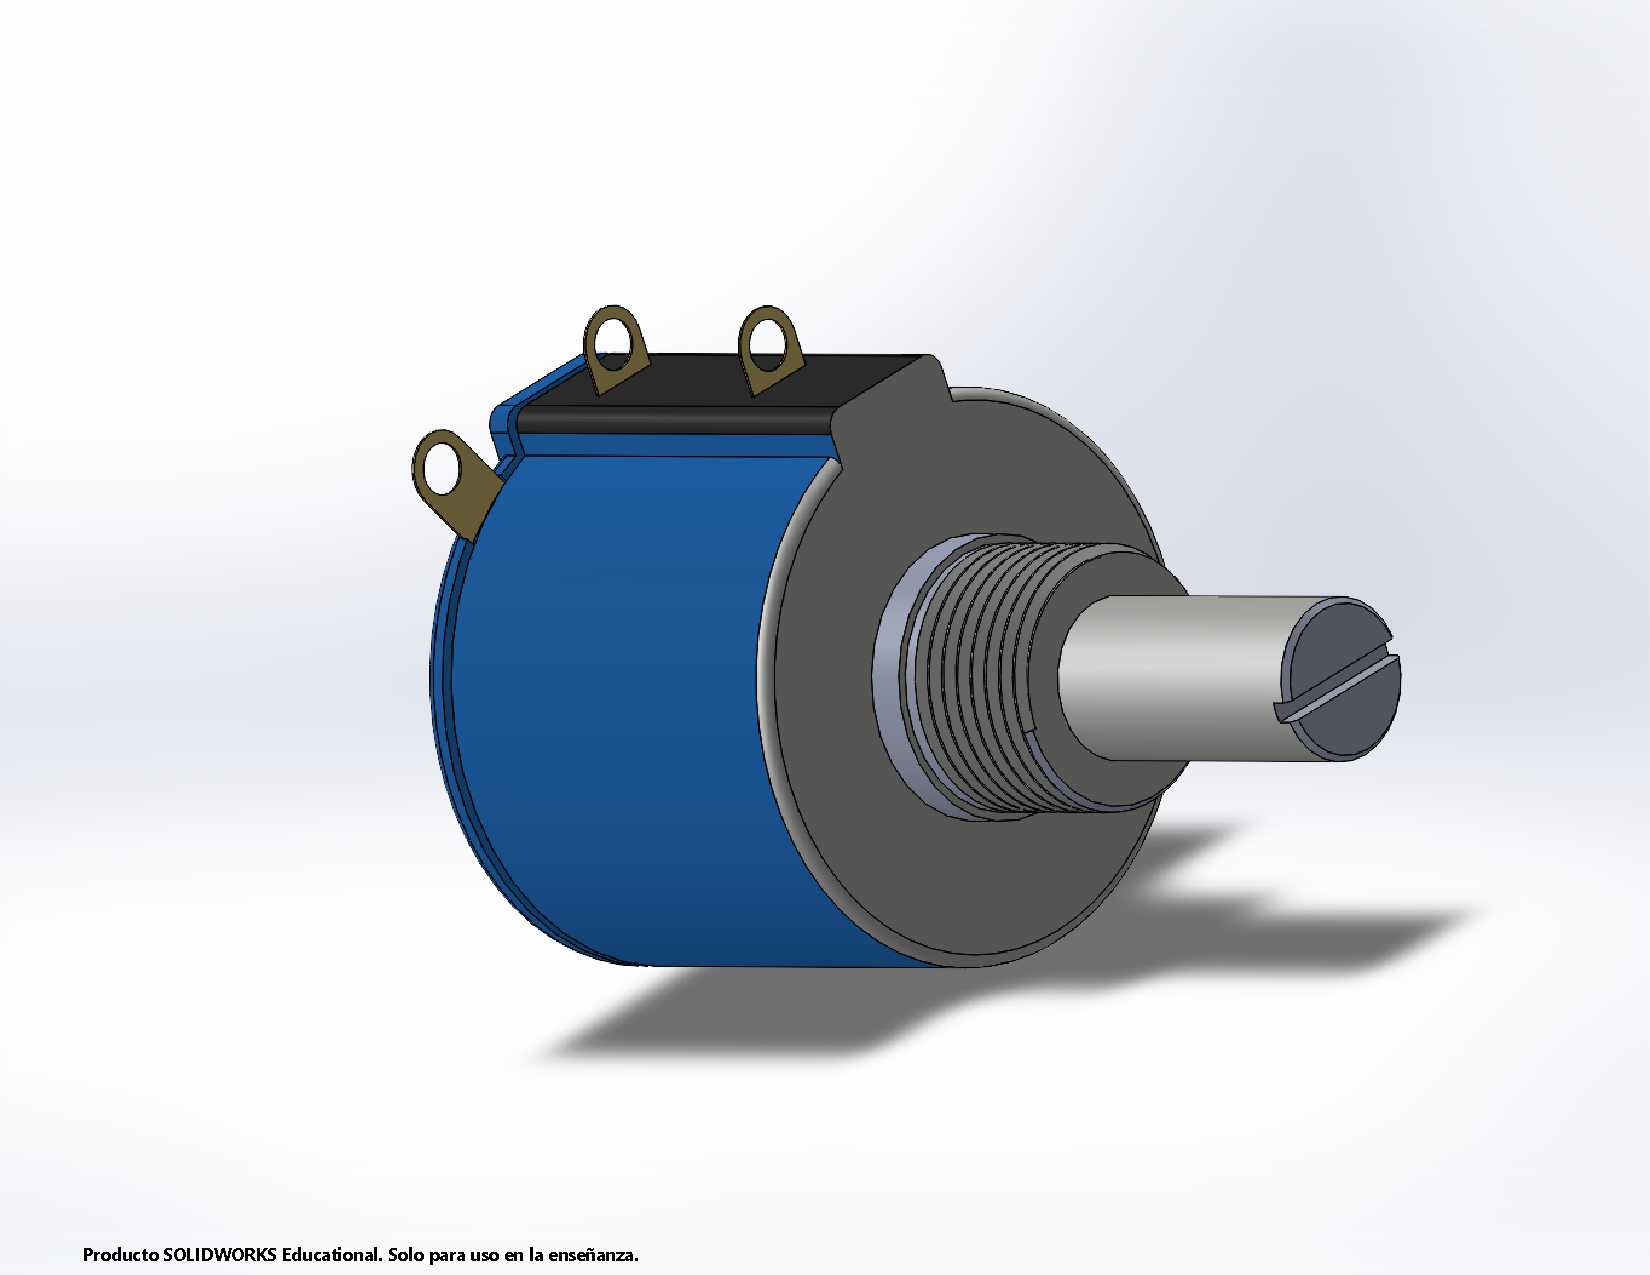
\includegraphics[width=.2\textwidth]{22/img/potenciometroFigura.PDF}~\\[5cm]  \end{center} & \\
     \hline
\end{tabular}

     
\begin{tabular}{ |p{1.5cm}|p{4cm}|p{4cm}|p{5cm}| }
\hline
 PC-07 & Resistencia  & \begin{center}
     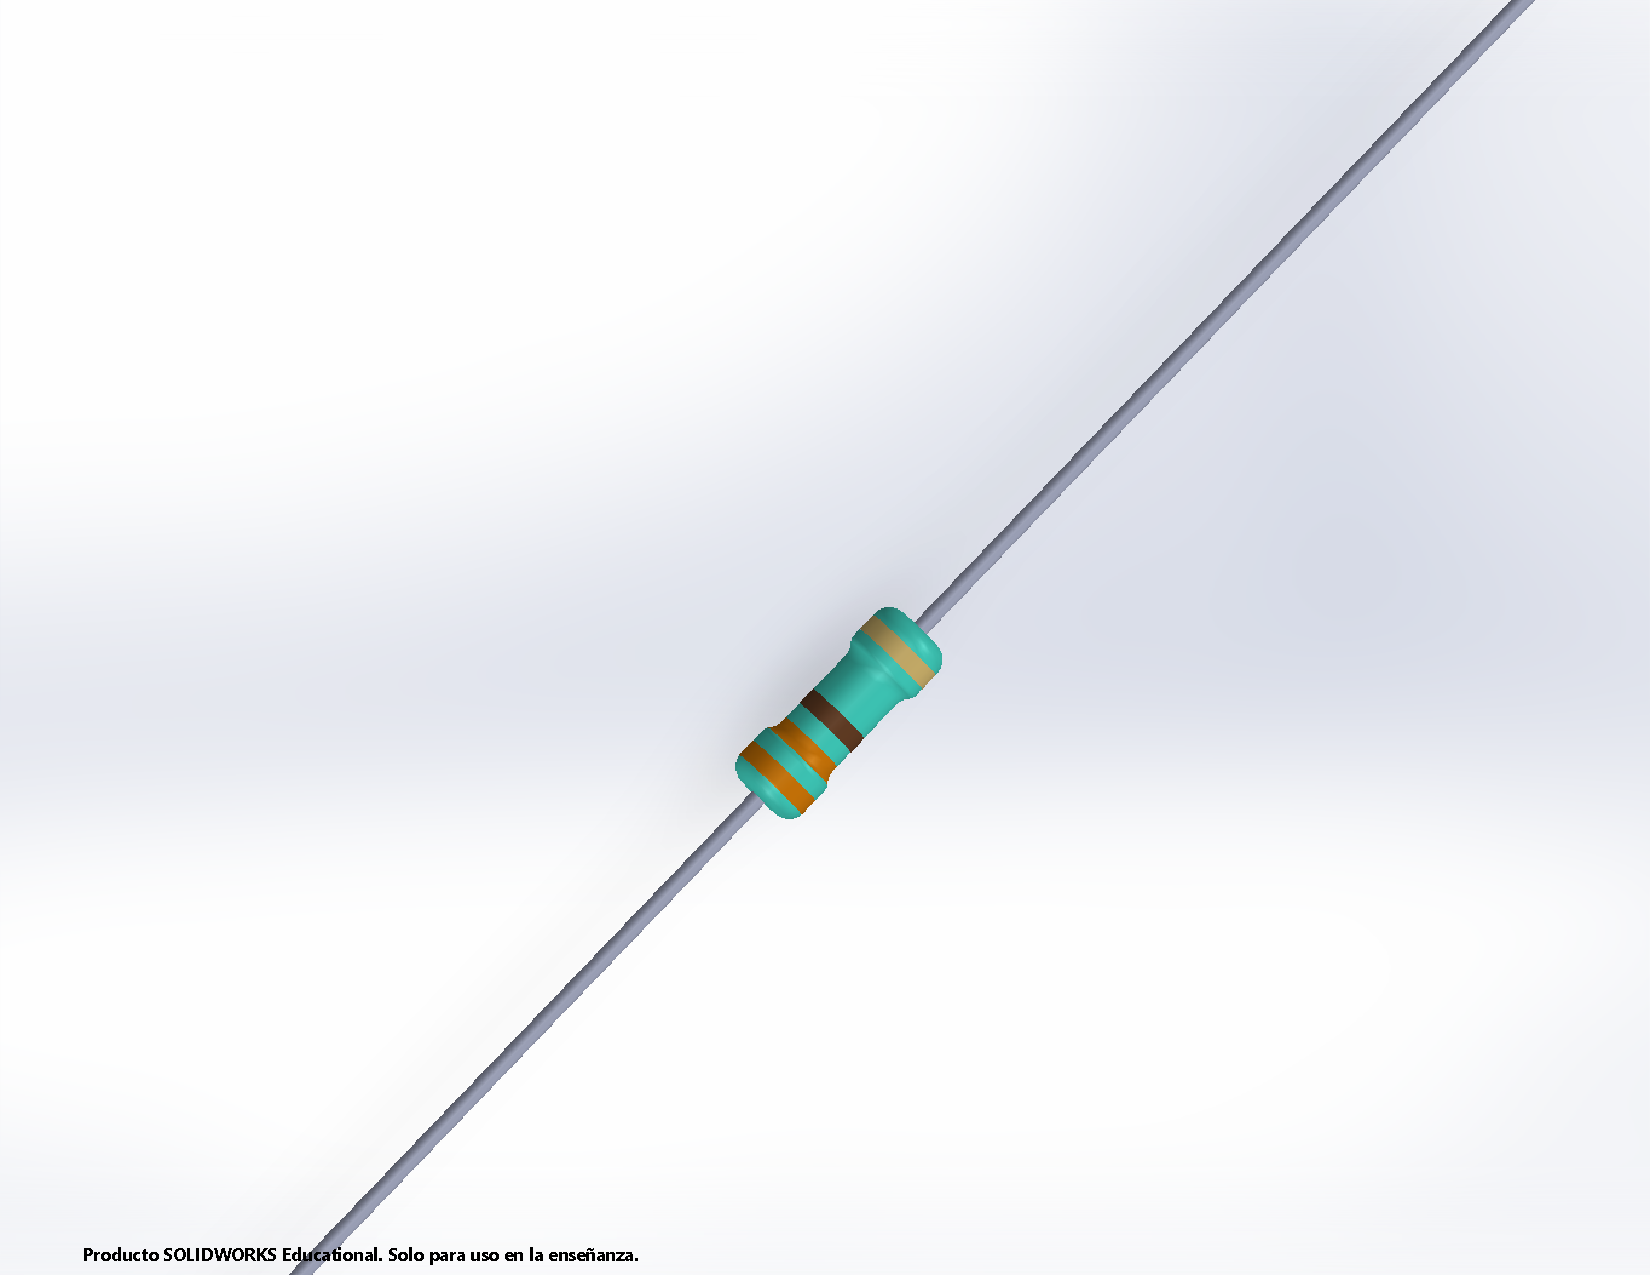
\includegraphics[width=.2\textwidth]{22/img/resistenciaFigura.PDF}~\\[5cm]  \end{center} &  \\
\hline
 PC-08 & Cable MH & \begin{center} 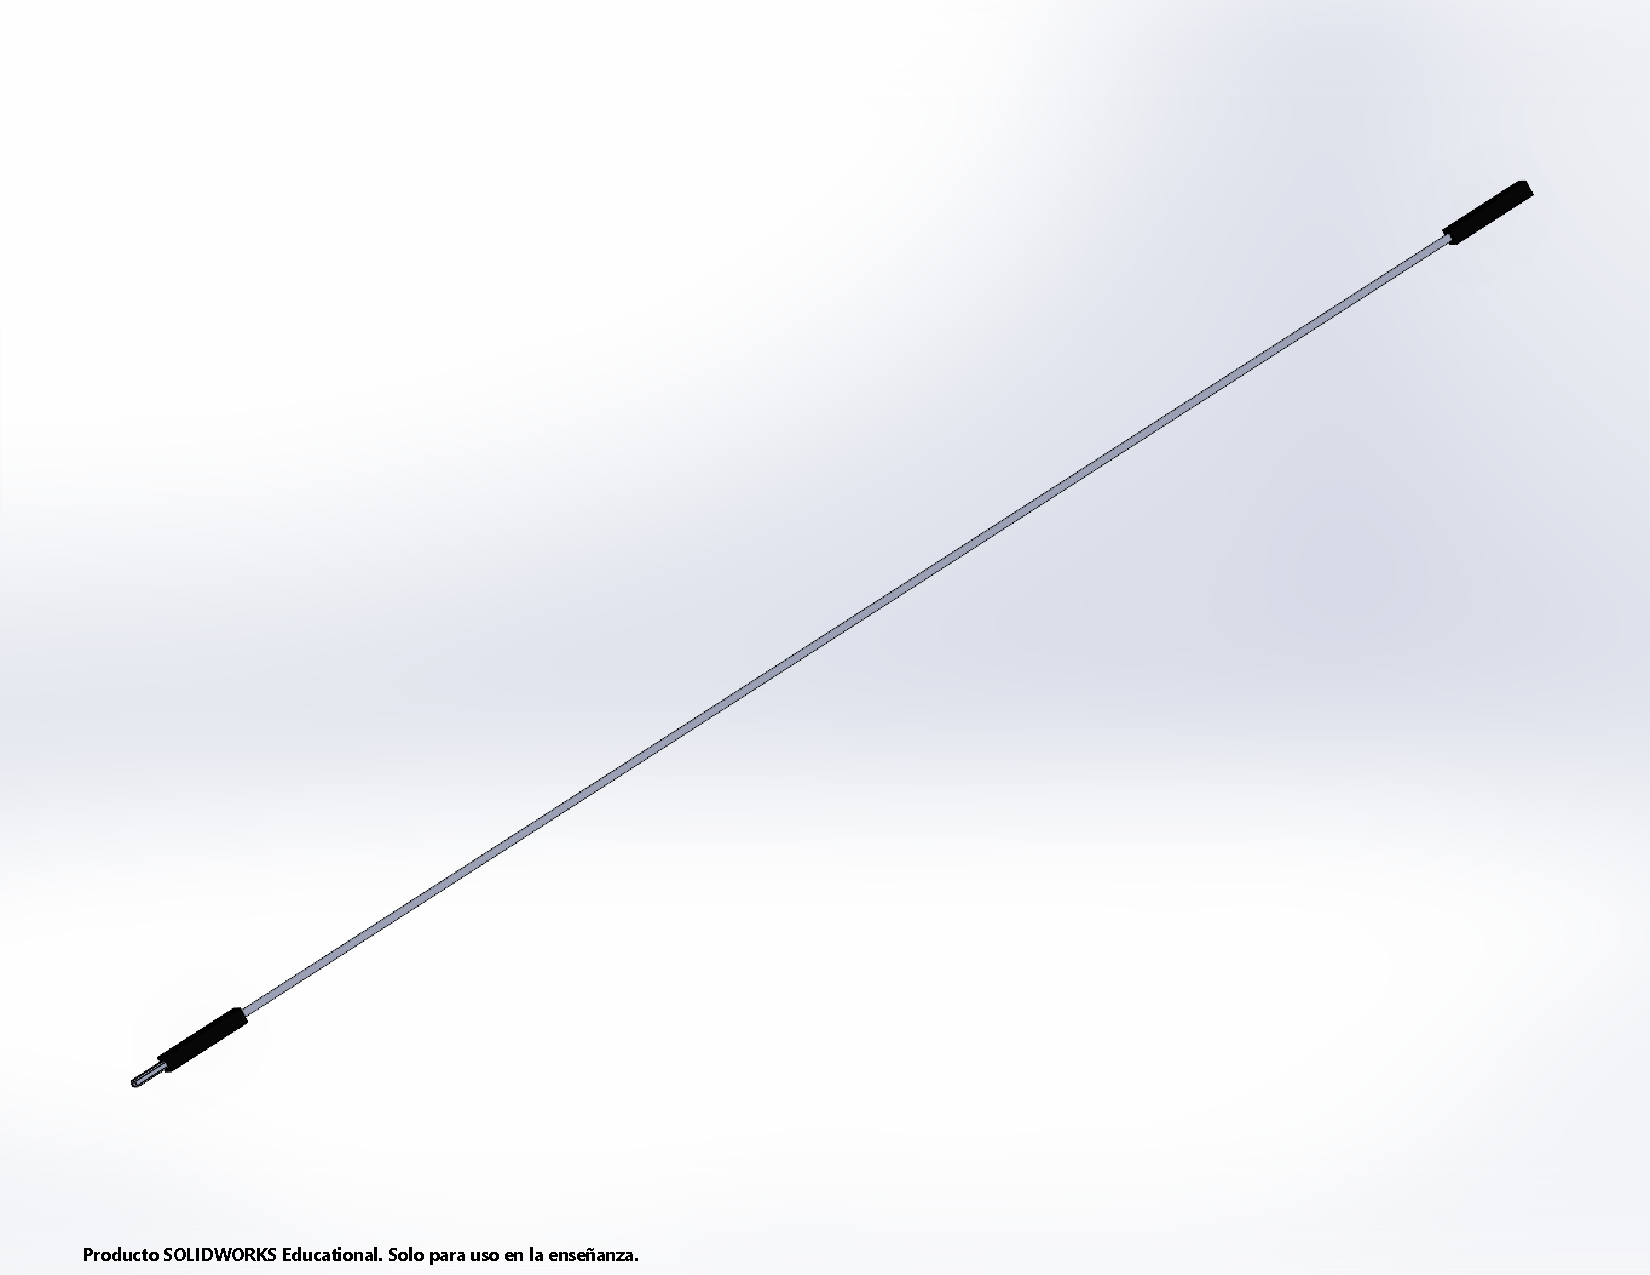
\includegraphics[width=.2\textwidth]{22/img/cableMHFigura.pdf}~\\[5cm] \end{center}  &  \\
\hline
PC-09 & Cable MM  & \begin{center} 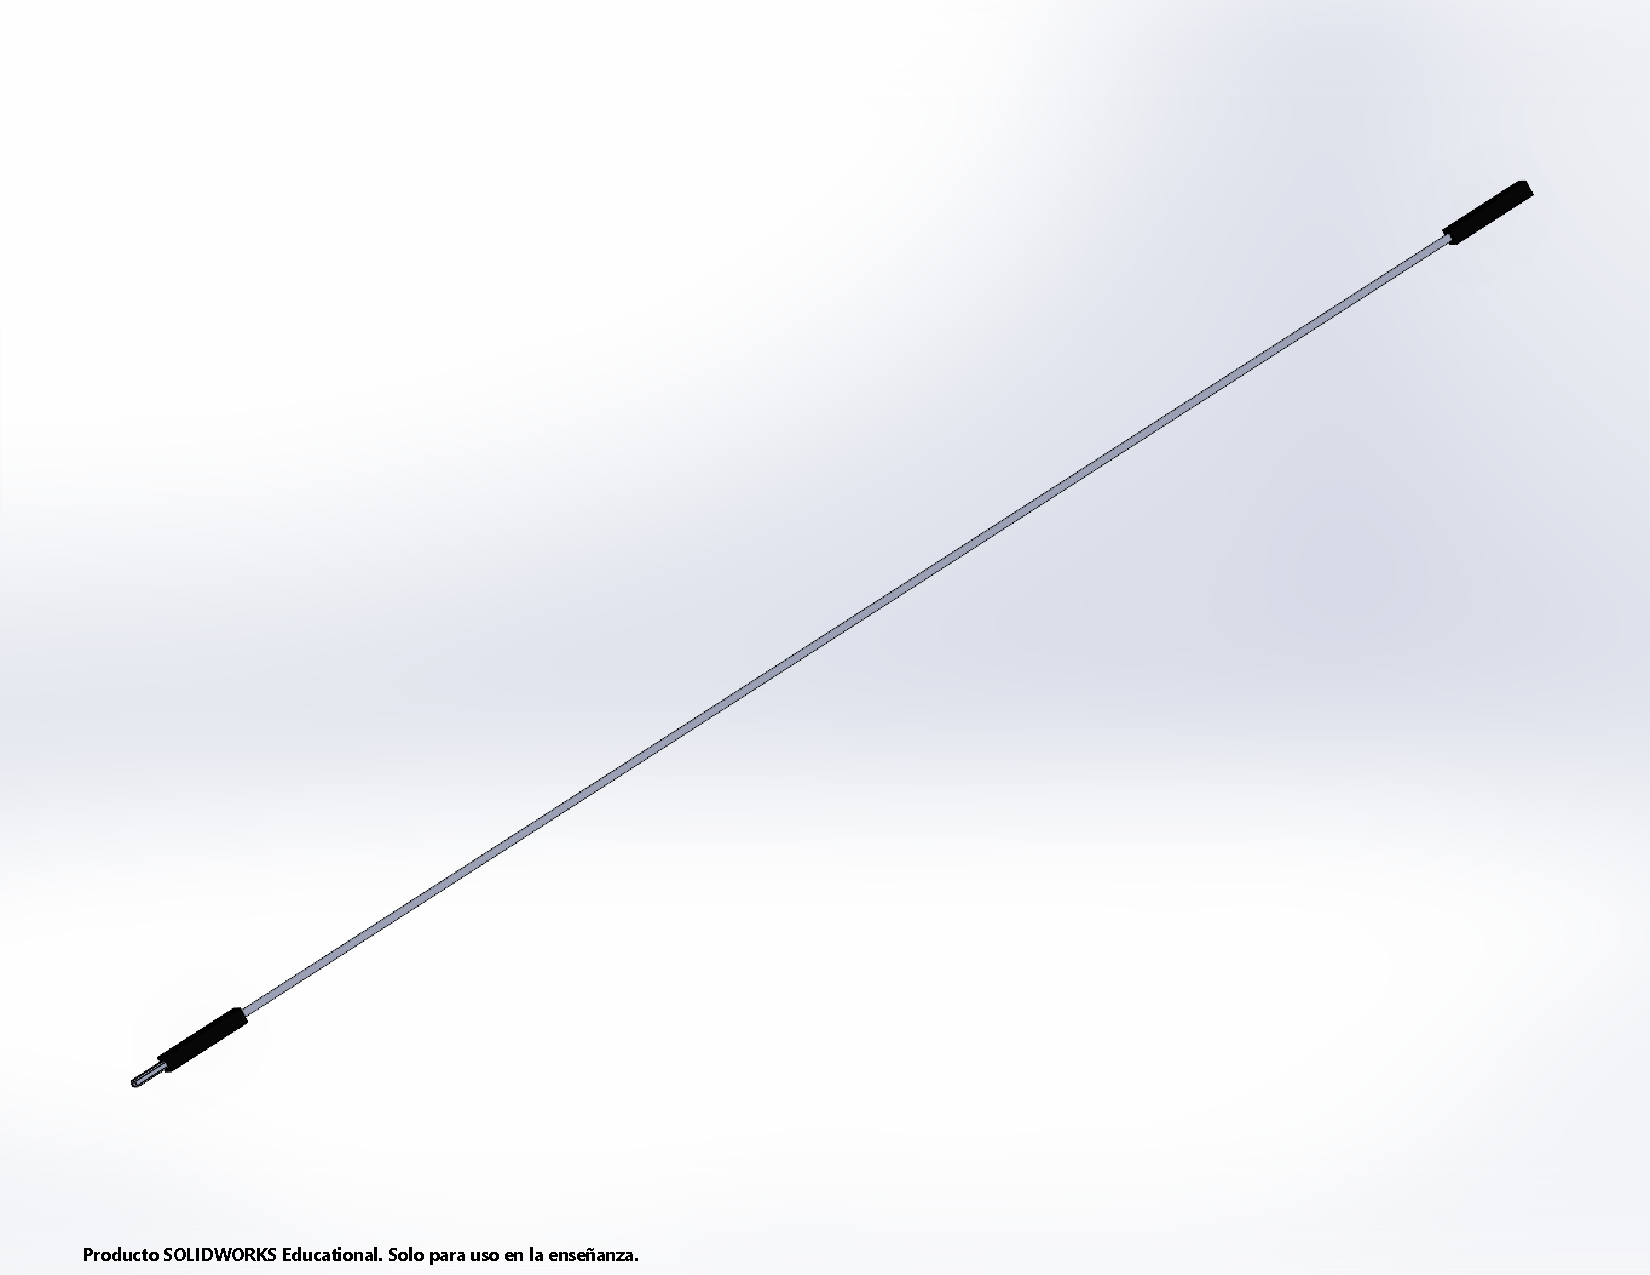
\includegraphics[width=.2\textwidth]{22/img/cableMHFigura.pdf}~\\[5cm] \end{center}  &  \\
\hline
 PC-10  & Multicontacto  &   & \\
\hline
 PC-11 & Cable de energía  &  &  \\
\hline


\end{tabular}

    
\end{center}


\begin{center}

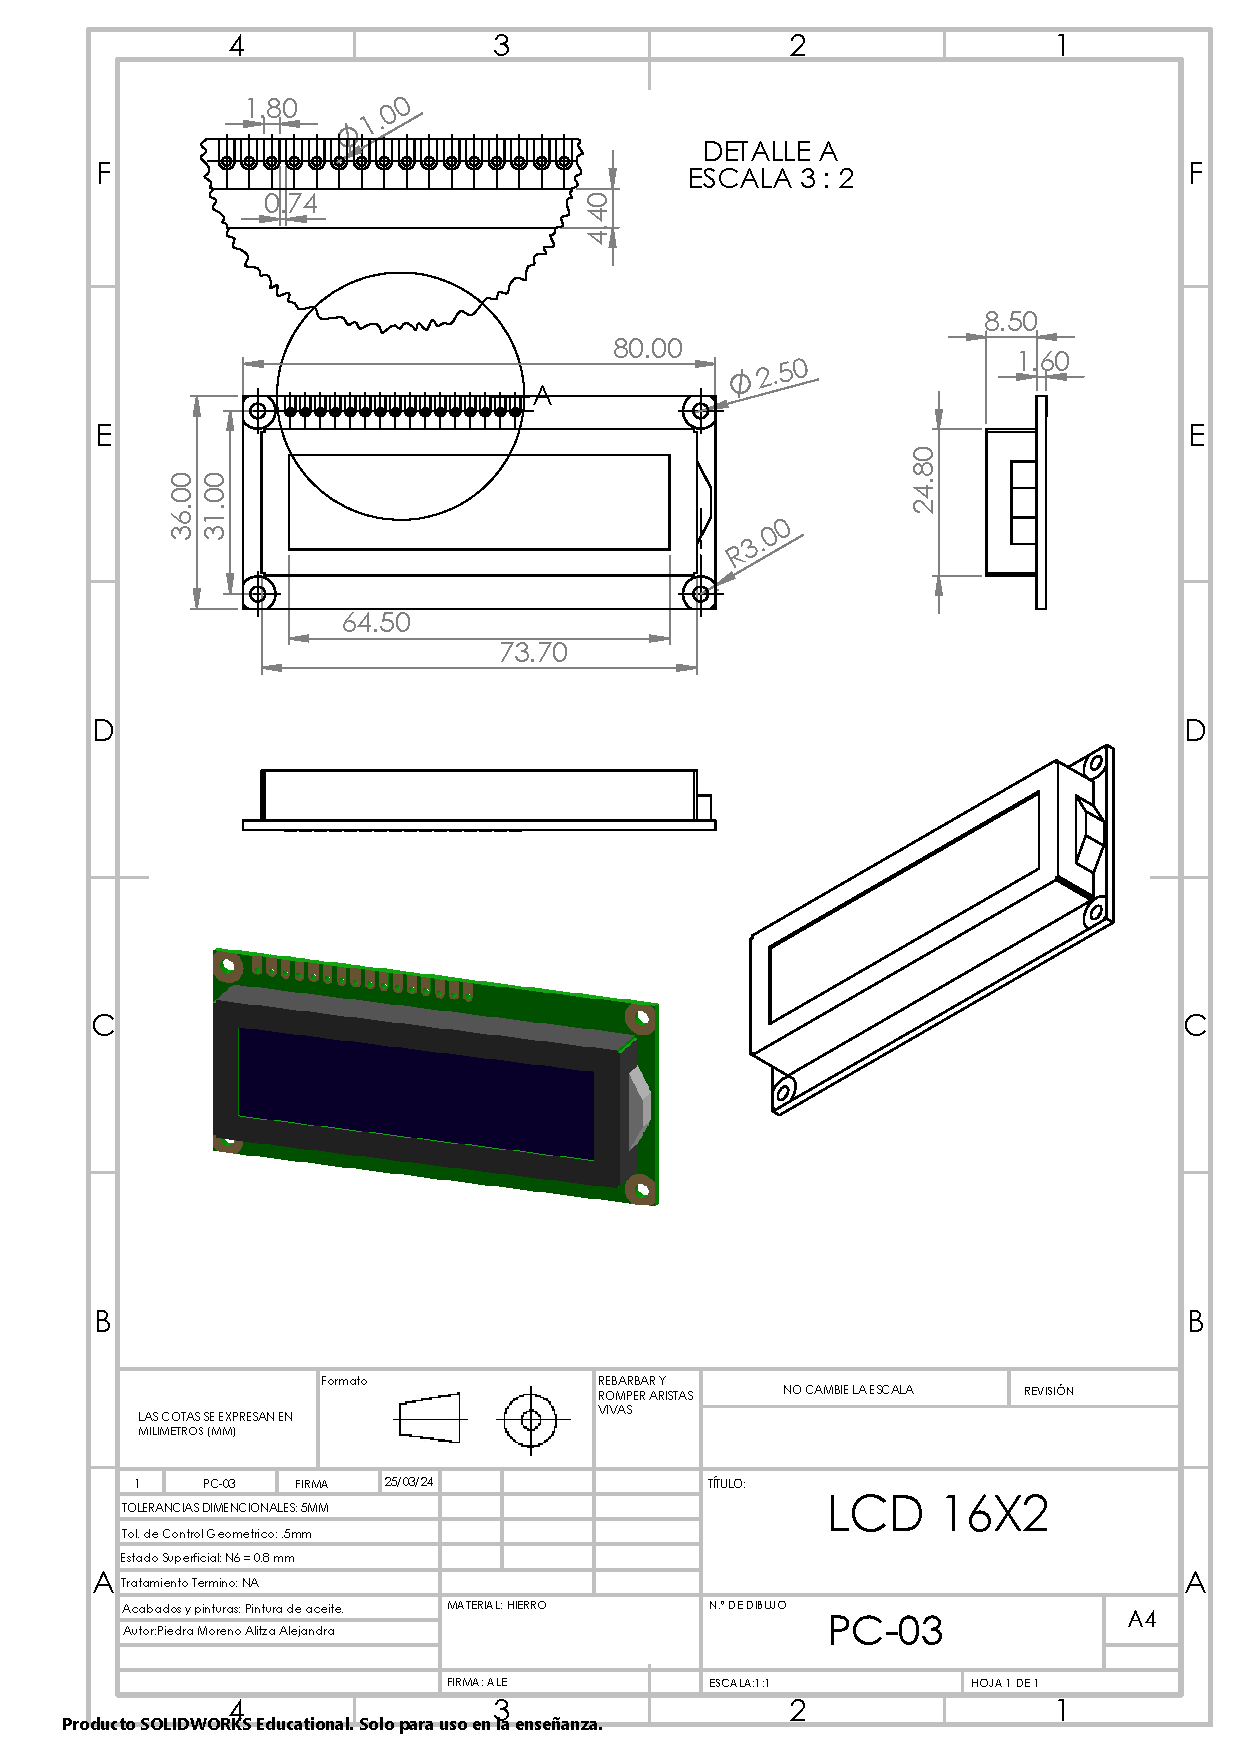
\includegraphics[width=.9\textwidth]{22/img/lcdDibujo.PDF}~\\[15cm]

\includegraphics[width=.9\textwidth]{22/img/móduloI2CInterfazDibujo.pdf}~\\[15cm]

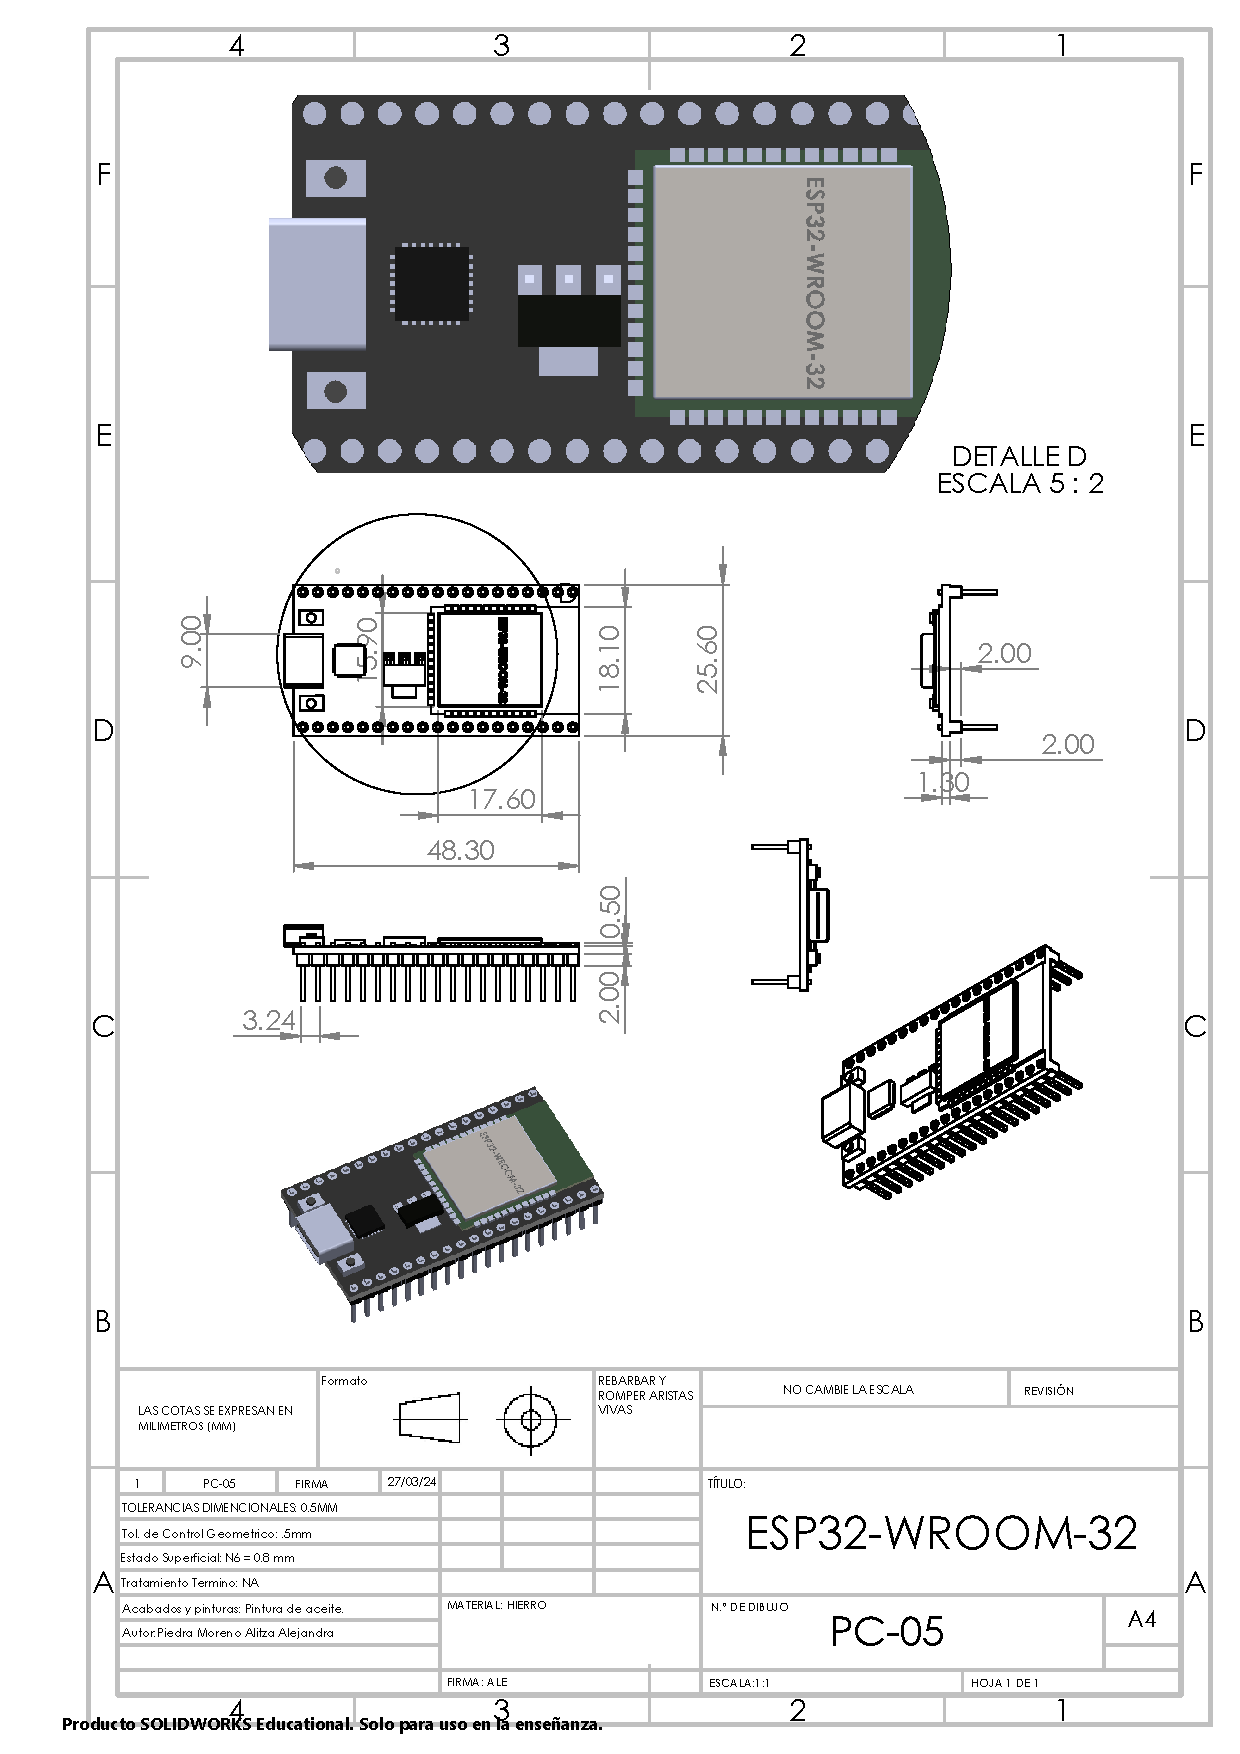
\includegraphics[width=.9\textwidth]{22/img/esp32Dibujo.pdf}~\\[15cm]

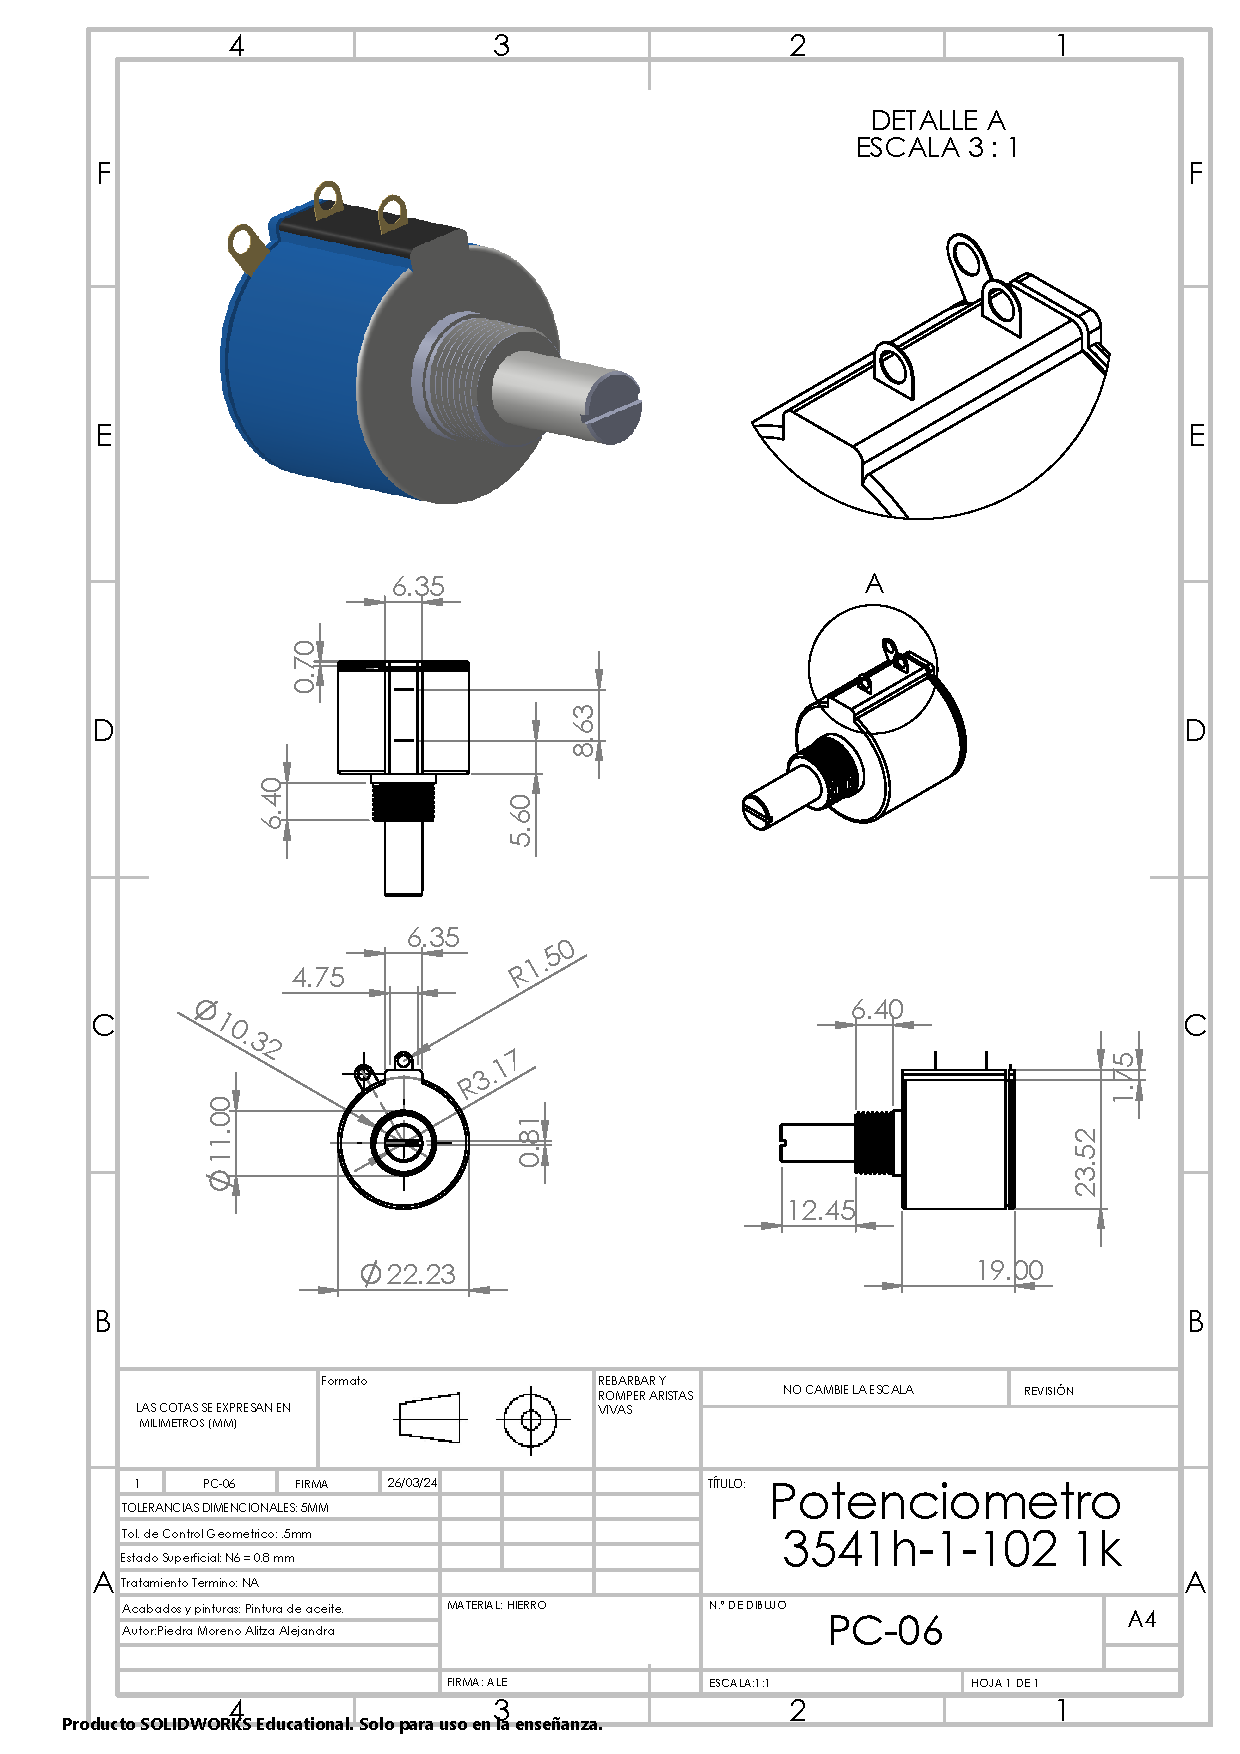
\includegraphics[width=.9\textwidth]{22/img/potenciometroDibujo.PDF}~\\[15cm]

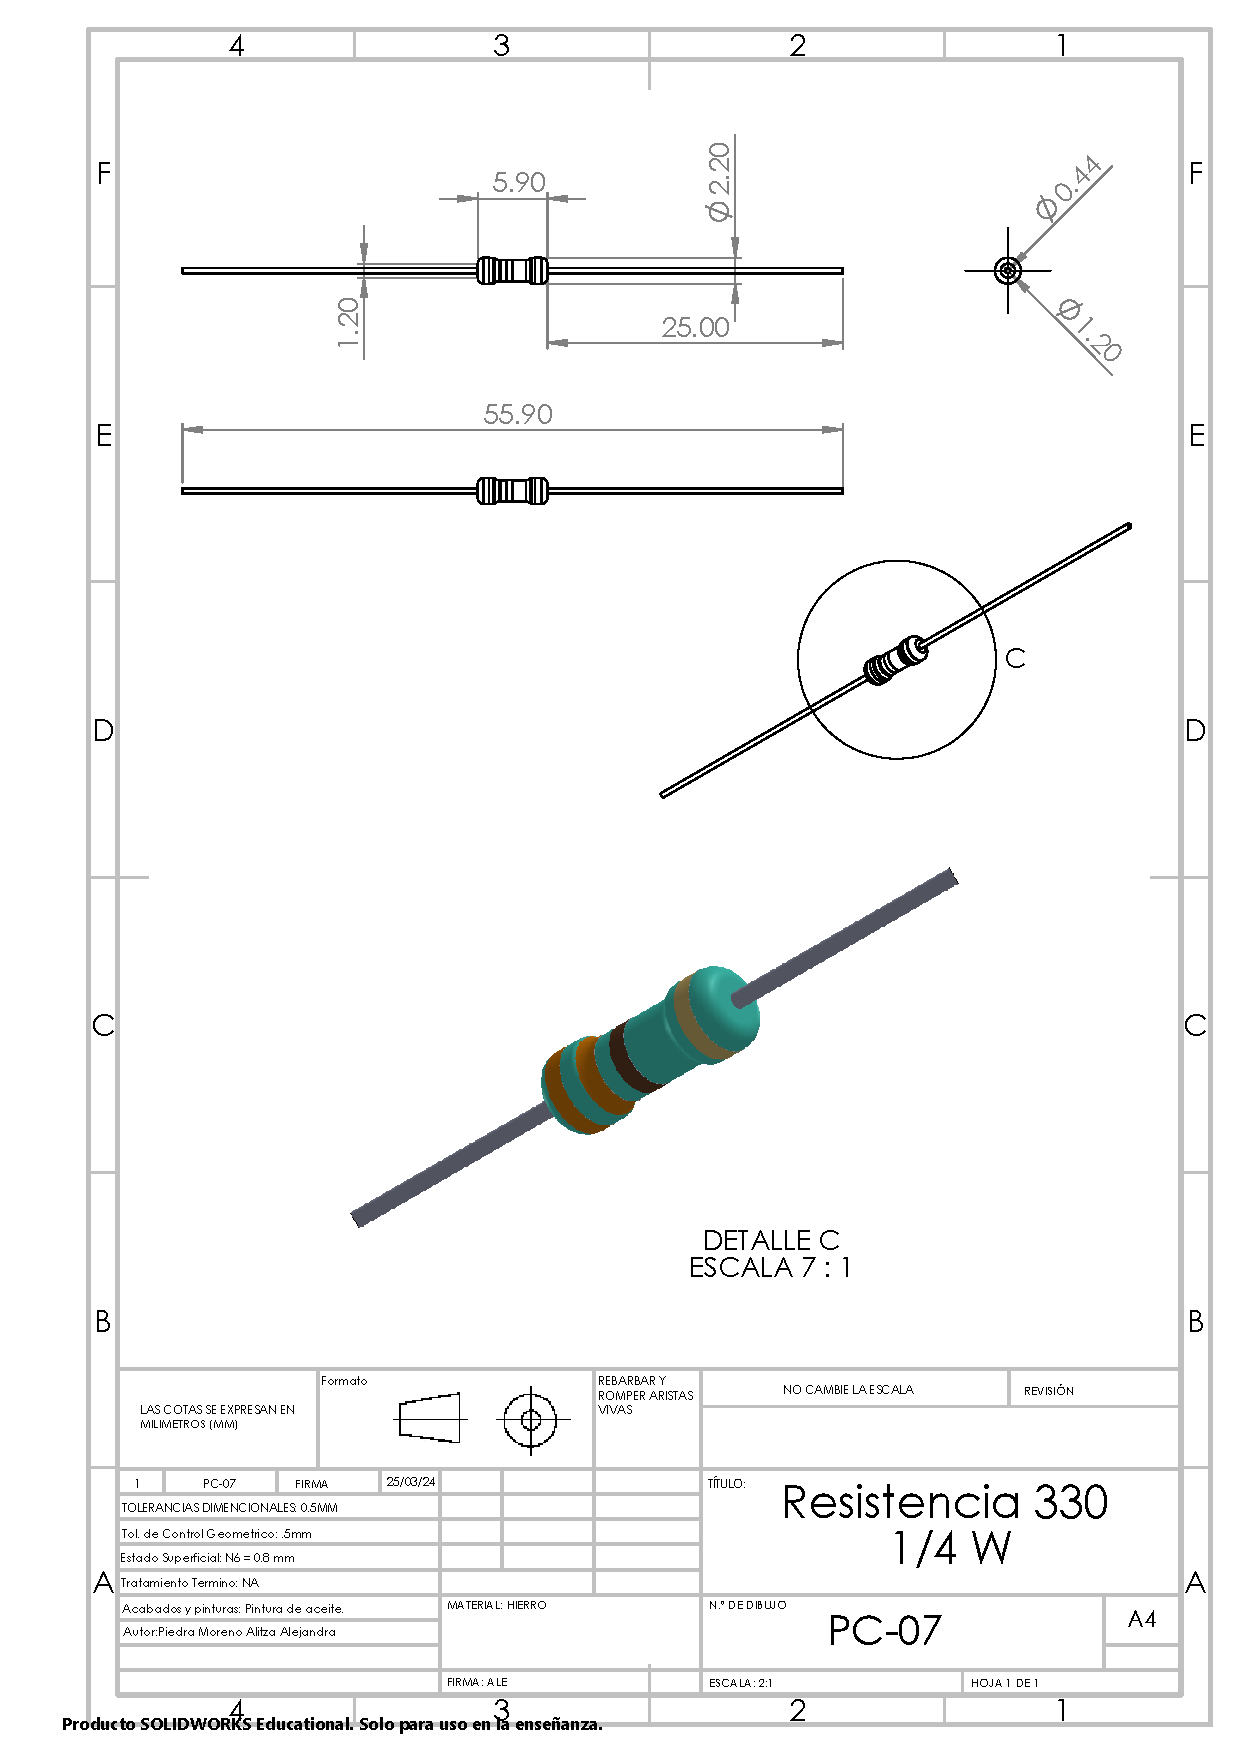
\includegraphics[width=.9\textwidth]{22/img/resistenciaDibujo.PDF}~\\[15cm]

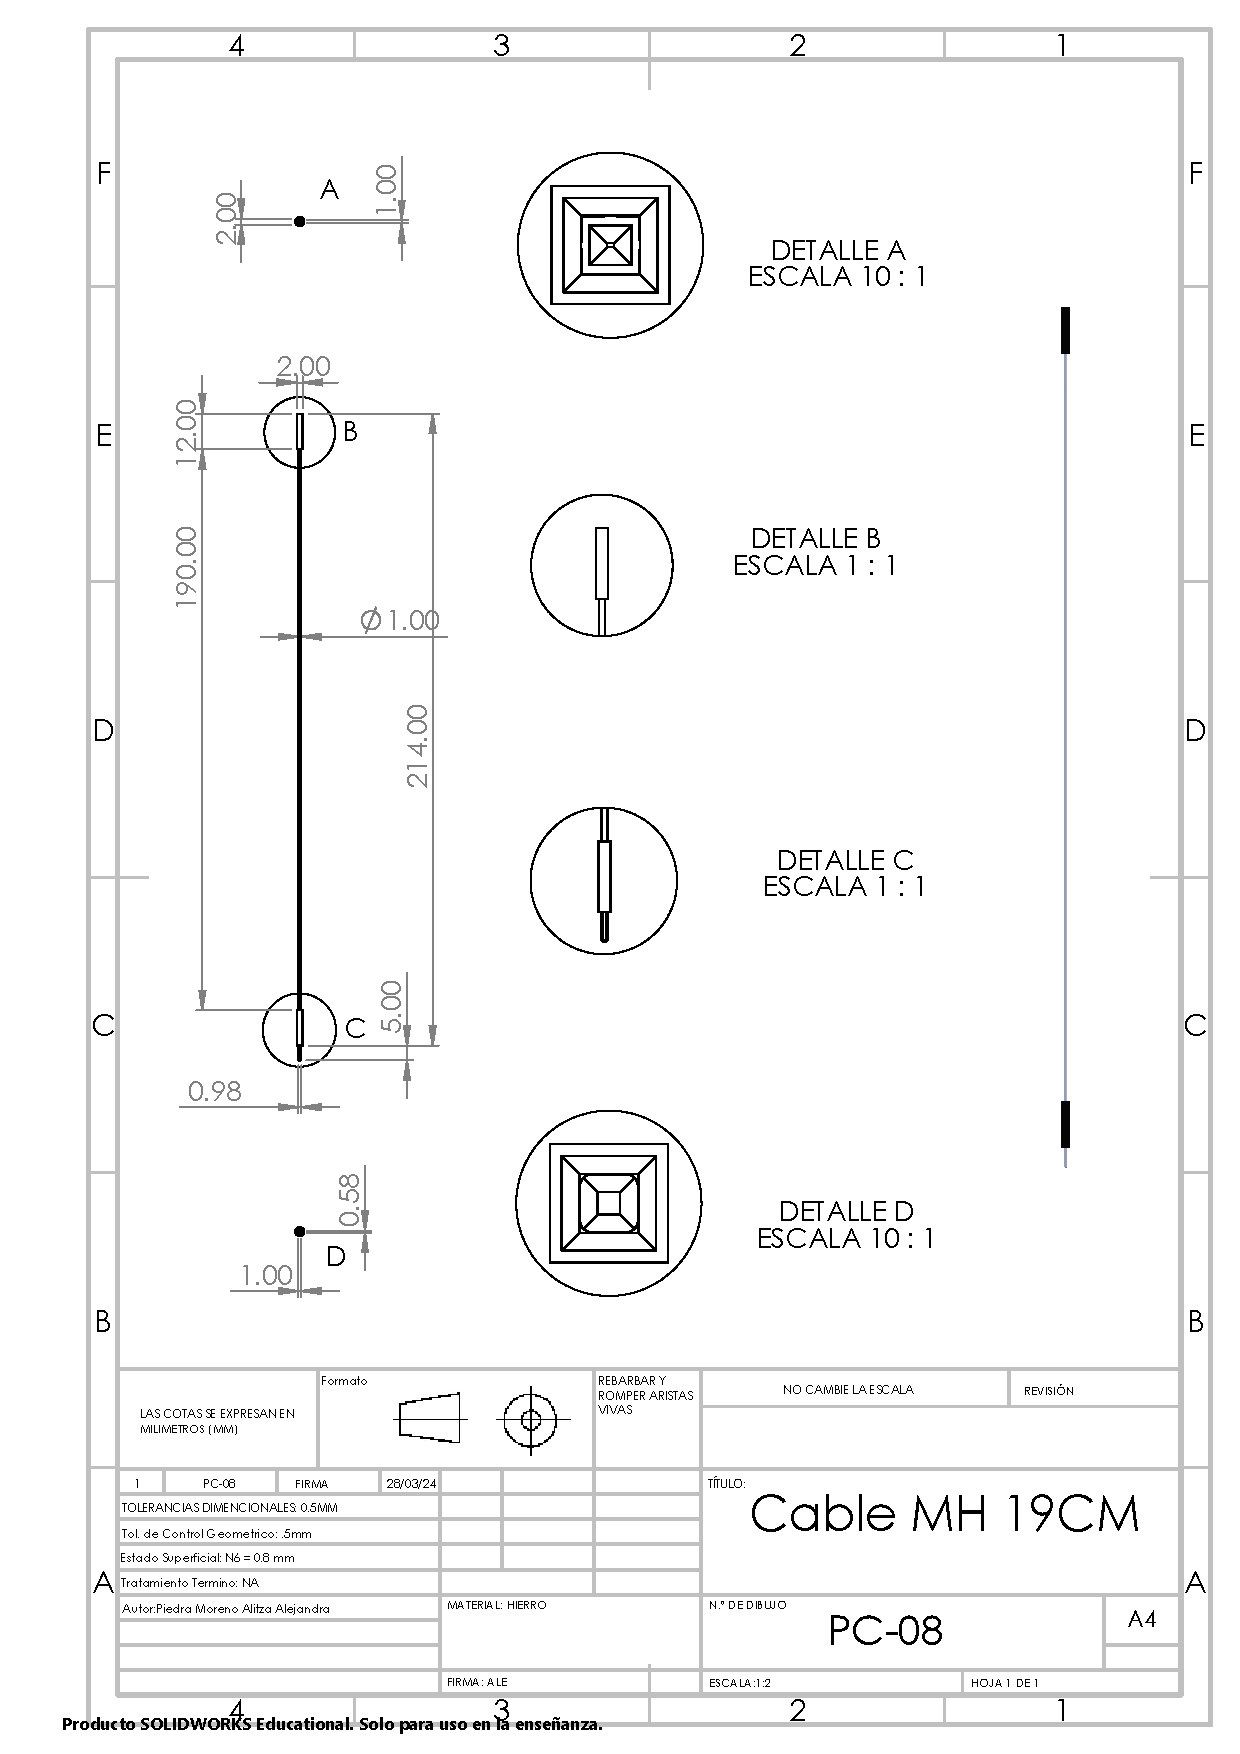
\includegraphics[width=.9\textwidth]{22/img/cableMHDibujo.PDF}~\\[15cm]

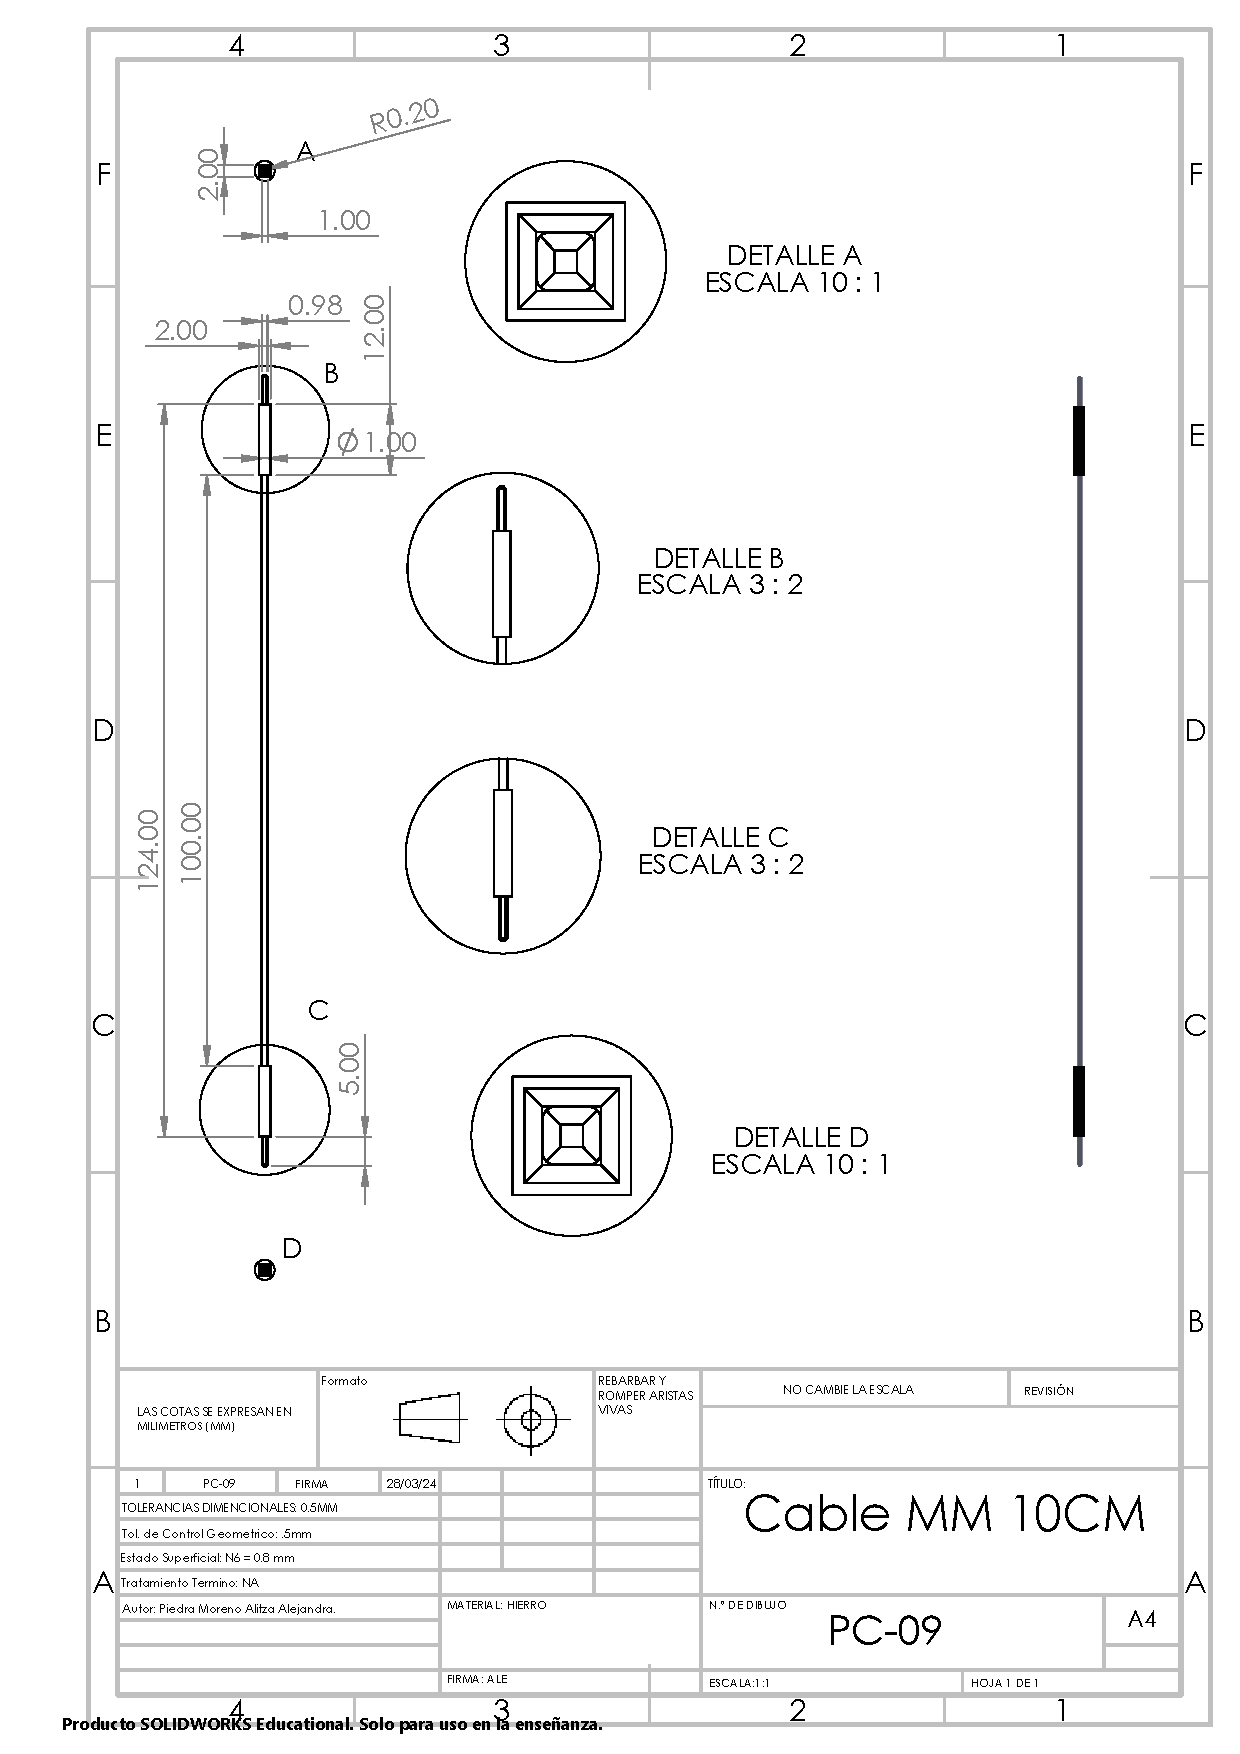
\includegraphics[width=.9\textwidth]{22/img/cableMMDibujo.PDF}~\\[15cm]

\end{center}



\bibliographystyle{apalike}
\bibliography{22/referencias}